% ============================================================
%  IntelliClave — AI Final Project Report (2 pages)
%  University of Engineering and Technology, Lahore
%  Institute of Data Sciences  |  Session 2024-2028
% ============================================================
\documentclass[10pt,a4paper,twocolumn]{article}

\usepackage[margin=1.25cm,top=1.2cm,bottom=1.25cm,columnsep=0.8cm]{geometry}
\usepackage{booktabs}
\usepackage{array}
\usepackage{tabularx}
\usepackage{enumitem}
\usepackage{tikz}
\usetikzlibrary{arrows.meta,positioning,fit,backgrounds,calc}
\usepackage[table]{xcolor}
\usepackage{titlesec}
\usepackage{microtype}
\usepackage{caption}

% ── Palette ─────────────────────────────────────────────────
\definecolor{accent}{RGB}{45,65,120}
\definecolor{accentlight}{RGB}{235,240,250}
\definecolor{clientblue}{RGB}{210,228,248}
\definecolor{serverorange}{RGB}{255,232,210}
\definecolor{teegreen}{RGB}{210,242,220}
\definecolor{rowalt}{RGB}{248,250,255}
\definecolor{goodgreen}{RGB}{20,100,60}
\definecolor{badred}{RGB}{160,40,40}

% ── Section headings ────────────────────────────────────────
\titleformat{\section}
  {\color{accent}\small\bfseries\sffamily\uppercase}
  {\thesection}{0.5em}{}
  [\vspace{1pt}{\color{accent}\titlerule[0.6pt]}\vspace{2pt}]
\titlespacing*{\section}{0pt}{7pt}{4pt}

\titleformat{\subsection}
  {\small\bfseries\sffamily\color{accent!85!black}}
  {}{0em}{}
\titlespacing*{\subsection}{0pt}{4pt}{2pt}

% ── Spacing & lists ─────────────────────────────────────────
\setlist[itemize]{
  noitemsep, topsep=2pt, parsep=0pt, partopsep=0pt,
  leftmargin=1.15em, label={\color{accent}\small\textbullet}
}
\setlength{\parskip}{2pt}
\setlength{\parindent}{0pt}
\setlength{\abovecaptionskip}{3pt}
\setlength{\belowcaptionskip}{2pt}
\renewcommand{\arraystretch}{1.15}
\captionsetup{font=small,labelfont={bf,color=accent},skip=3pt}

% ── Helpers ─────────────────────────────────────────────────
\newcommand{\resistant}{\textcolor{goodgreen}{\textbf{Resistant}}}
\newcommand{\vulnerable}{\textcolor{badred}{\textbf{Vulnerable}}}
\newcommand{\passed}{\textcolor{goodgreen}{\textbf{Passed}}}

\newenvironment{keybox}{%
  \vspace{2pt}%
  \noindent\colorbox{accentlight}{%
    \begin{minipage}{\dimexpr\columnwidth-2\fboxsep}%
      \vspace{4pt}\small%
}{%
      \vspace{4pt}%
    \end{minipage}%
  }%
  \vspace{3pt}%
}

% ============================================================
\begin{document}

% ── Full-width title block ──────────────────────────────────
\twocolumn[{%
\begin{center}
  \color{accent}\rule{\textwidth}{1.2pt}\\[6pt]
  {\LARGE\bfseries\sffamily\color{black}
    IntelliClave}\\[2pt]
  {\large\bfseries\sffamily\color{accent!80!black}
    Privacy-Preserving Federated Learning for Human Activity Recognition}\\[1pt]
  {\small\sffamily\color{black}
    via Confidential Computing \textbar{} Differential Privacy \textbar{} Encrypted FL}\\[8pt]

  \begin{tabular}{@{}c@{\hspace{1.8em}}c@{\hspace{1.8em}}c@{\hspace{1.8em}}c@{}}
    \textbf{Amna Naveed} & \textbf{Fatima Ambreen} & \textbf{Zartashia Naz} & \textbf{Armeen Asim} \\
    {\footnotesize 2024-DS-42} & {\footnotesize 2024-DS-52} & {\footnotesize 2024-DS-13} & {\footnotesize 2024-DS-44} \\
  \end{tabular}\\[6pt]

  {\small\itshape
    Institute of Data Sciences, University of Engineering and Technology, Lahore\\
    Session 2024--2028 \quad\textbar\quad Course: Artificial Intelligence}
  \vspace{4pt}
  \color{accent}\rule{\textwidth}{0.5pt}
  \vspace{8pt}
\end{center}
}]

% ============================================================
\section{Motivation}
Healthcare and fitness organisations collect complementary smartphone inertial-sensor data, but regulations (GDPR, HIPAA, PMDC) forbid centralising raw records. Training only on local data produces weak models---especially for minority activity classes under non-IID splits. \textbf{IntelliClave} enables privacy-compliant collaboration: each site keeps its data local, shares only noised model updates, and relies on encrypted transport plus attested server aggregation.

% ============================================================
\section{Problem Statement}
Given three organisations with \textbf{non-IID} UCI HAR windows (10{,}299 samples, 561 features, 6 classes), learn a shared activity classifier satisfying:
\textbf{(i)}~no raw data exchange;
\textbf{(ii)}~$(\varepsilon,\delta)$-differential privacy on client updates;
\textbf{(iii)}~AES-256-GCM encrypted gradients and verifiable TEE attestation at the server;
\textbf{(iv)}~quantified utility and security versus explicit baselines (solo DP training, attack simulations).

% ============================================================
\section{Dataset \& Methodology}

\subsection{Input data}
UCI HAR (Anguita et al., 2013): waist-mounted Samsung Galaxy S\,II, 50\,Hz accelerometer/gyroscope, 2.56\,s windows (50\,\% overlap). Classes: \textit{WALKING, WALKING\_UPSTAIRS, WALKING\_DOWNSTAIRS, SITTING, STANDING, LAYING}. We partition with \textbf{Dirichlet} ($\alpha{=}0.5$, 3 clients, \textbf{no PCA}---full 561-dim features).

\begin{table}[h!]
\centering
\caption{Non-IID client distribution (Dirichlet $\alpha{=}0.5$)}
\small
\rowcolors{2}{rowalt}{white}
\begin{tabular}{@{}lrrrrrrr@{}}
\toprule
\textbf{Client} & \textbf{Samples} & \textbf{L0} & \textbf{L1} & \textbf{L2} & \textbf{L3} & \textbf{L4} & \textbf{L5} \\
\midrule
Client 1 & 5{,}529 & 1{,}494 & 1{,}184 & 401 & 785 & 782 & 883 \\
Client 2 & 2{,}288 & 27 & 331 & 651 & 238 & 8 & 1{,}033 \\
Client 3 & 2{,}482 & 201 & 29 & 354 & 754 & 1{,}116 & 28 \\
\bottomrule
\end{tabular}
\end{table}

\subsection{Model \& training stack}
\textbf{Classifier:} PyTorch \texttt{FLClassifier} MLP: $561 \!\to\! 96 \!\to\! 48 \!\to\! 6$ (ReLU, dropout $p{=}0.5$, class-weighted CrossEntropyLoss).

\begin{table}[h!]
\centering
\caption{Secure FL training configuration (reference run)}
\small
\rowcolors{2}{rowalt}{white}
\begin{tabular}{@{}ll@{}}
\toprule
\textbf{Parameter} & \textbf{Value} \\
\midrule
FL framework / strategy & Flower 1.6.0 / \textbf{FedProx} \\
Rounds / clients / local epochs & 35 / 3 / 1 \\
Batch size / optimiser & 64 / Adam ($lr{=}10^{-3}$) \\
DP engine & Opacus DP-SGD ($\varepsilon_{\text{target}}{=}8$, $\delta{=}1/n$) \\
Max grad norm & 0.3 \\
Privacy consumed & $\varepsilon \approx 7.99$ \\
Crypto \& attestation & AES-256-GCM + TLS\,1.3 + Gramine demo \\
Inference defence & PrivacyWrapper (noise 0.5, temp.\ 1.0) \\
\bottomrule
\end{tabular}
\end{table}

\subsection{System workflow}
\begin{center}
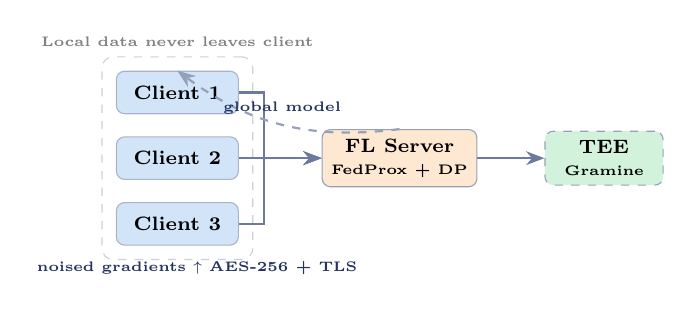
\begin{tikzpicture}[
  node distance=0.32cm and 0.55cm,
  client/.style={draw=accent!40, rounded corners=3pt, fill=clientblue,
    minimum width=1.55cm, minimum height=0.54cm,
    font=\scriptsize\bfseries, align=center},
  server/.style={draw=accent!50, rounded corners=3pt, fill=serverorange,
    minimum width=1.65cm, minimum height=0.62cm,
    font=\scriptsize\bfseries, align=center},
  tee/.style={draw=accent!50, dashed, rounded corners=3pt, fill=teegreen,
    minimum width=1.5cm, minimum height=0.54cm,
    font=\scriptsize\bfseries, align=center},
  arr/.style={-Stealth, thick, accent!70},
  lbl/.style={font=\tiny, text=accent!80!black}
]
\node[client] (c1) {Client 1};
\node[client, below=0.28cm of c1] (c2) {Client 2};
\node[client, below=0.28cm of c2] (c3) {Client 3};
\node[server, right=1.05cm of c2] (fl) {FL Server\\{\tiny FedProx + DP}};
\node[tee, right=0.85cm of fl] (tee) {TEE\\{\tiny Gramine}};
\draw[arr] (c1.east) -- ++(0.32,0) |- (fl.west);
\draw[arr] (c2.east) -- (fl.west);
\draw[arr] (c3.east) -- ++(0.32,0) |- (fl.west);
\draw[arr] (fl.east) -- (tee.west);
\draw[arr, dashed, accent!50, bend left=22]
  (fl.north) to node[lbl, above]{\textbf{global model}} (c1.north);
\node[lbl, below=0.08cm of c3, xshift=0.25cm]
  {\textbf{noised gradients} $\uparrow$ \textbf{AES-256 + TLS}};
\begin{scope}[on background layer]
  \node[draw=accent!25, dashed, inner sep=5pt, rounded corners=4pt,
    fit=(c1)(c2)(c3),
    label={[lbl,gray]above:\textbf{Local data never leaves client}}] {};
\end{scope}
\end{tikzpicture}
\end{center}

% ============================================================
\section{Evaluation Criteria}
We compare methods that answer different research questions---not a single accuracy leaderboard:

\begin{itemize}
  \item \textbf{Solo local + DP} --- sites train in isolation (collaboration lower bound).
  \item \textbf{Global FL + DP (ours)} --- primary secure federated system.
  \item \textbf{Attack baselines} --- FedAvg under 100\,\% label-flip vs.\ trimmed-mean mitigation.
  \item \textbf{Centralised training} --- excluded (violates data-sovereignty constraints).
\end{itemize}
\textbf{Metrics:} accuracy, macro F1, $\varepsilon$; attack AUC, accuracy drop, cosine similarity.

\subsection{Utility comparison}
\begin{table}[h!]
\centering
\caption{Privacy--utility baselines (DP-matched solo vs.\ federated)}
\small
\rowcolors{2}{rowalt}{white}
\begin{tabular}{@{}lccc@{}}
\toprule
\textbf{Method} & \textbf{Acc (\%)} & \textbf{Macro F1} & \textbf{$\varepsilon$} \\
\midrule
Solo local + DP (weighted) & 78.9 & 0.528 & $\leq 10$ \\
\rowcolor{accentlight}
\textbf{Global FL + DP (ours)} & \textbf{85.0} & \textbf{0.780} & \textbf{7.99} \\
\bottomrule
\multicolumn{4}{@{}l@{}}{\footnotesize Collaboration gain: \textbf{+32.9\,pp} weighted macro F1 (3/3 clients improved)} \\
\end{tabular}
\end{table}

\begin{table}[h!]
\centering
\caption{Per-client macro F1: solo local vs.\ global FL (DP-matched)}
\small
\rowcolors{2}{rowalt}{white}
\begin{tabular}{@{}lccc@{}}
\toprule
\textbf{Client} & \textbf{Solo F1} & \textbf{Global F1} & \textbf{$\Delta$ F1} \\
\midrule
Client 1 & 0.577 & 0.928 & +35.1\,pp \\
Client 2 & 0.603 & 0.729 & +12.7\,pp \\
Client 3 & 0.351 & 0.817 & +46.6\,pp \\
\bottomrule
\end{tabular}
\end{table}

\subsection{Security evaluation}
\begin{table}[h!]
\centering
\caption{Attack simulation results on trained global model}
\small
\rowcolors{2}{rowalt}{white}
\begin{tabular}{@{}p{2.1cm}p{1.55cm}cc@{}}
\toprule
\textbf{Attack} & \textbf{Setting} & \textbf{Metric} & \textbf{Verdict} \\
\midrule
Membership inference & DP model & AUC 0.505 & \resistant \\
Model inversion & PrivacyWrapper & cos.\ sim.\ 0.017 & \resistant \\
Grad.\ poisoning & FedAvg, 100\% flip & $-$76.8\% acc & \vulnerable \\
Grad.\ poisoning & Trimmed mean & $-$1.0\% acc & \resistant \\
Crypto / attestation & Self-tests & 4/4; rogue blocked & \passed \\
\bottomrule
\end{tabular}
\end{table}

\begin{keybox}
\textbf{Main result:} Under non-IID Dirichlet data and $\varepsilon \approx 8$, secure FL reaches \textbf{85.0\,\%} accuracy with \textbf{0.78} macro F1, outperforming solo DP models on every client. DP keeps membership AUC near random ($\approx 0.5$); PrivacyWrapper blocks inversion; trimmed-mean aggregation limits Byzantine label-flips in simulation.
\end{keybox}

% ============================================================
\section{Hardware \& Tools}

\begin{table}[h!]
\centering
\caption{Training hardware}
\small
\rowcolors{2}{rowalt}{white}
\begin{tabular}{@{}p{2.2cm}p{4.7cm}@{}}
\toprule
\textbf{Component} & \textbf{Specification} \\
\midrule
Processor & Intel Core i7-1355U (13th Gen), \textbf{CPU-only} --- no GPU \\
Host OS & Windows 11; Python 3.10 (\texttt{conda} env \texttt{intelliclave}) \\
TEE runtime & Gramine \texttt{gramine-direct} on WSL2 Ubuntu 22.04 \\
SGX hardware & Not on laptop (simulated attestation) \\
Deployment & Docker Compose; Minikube Kubernetes (single-node) \\
\bottomrule
\end{tabular}
\end{table}

\begin{table}[h!]
\centering
\caption{Software stack}
\small
\rowcolors{2}{rowalt}{white}
\begin{tabular}{@{}p{2cm}p{4.9cm}@{}}
\toprule
\textbf{Layer} & \textbf{Technologies} \\
\midrule
ML / data & PyTorch 2.1.0, scikit-learn, NumPy, Pandas \\
Federated FL & Flower 1.6.0 (FedProx) \\
Privacy & Opacus 1.4.0 (DP-SGD, RDP accountant) \\
Crypto / TEE & PyCryptodome, pyOpenSSL, Gramine 1.9 \\
API / UI & FastAPI 0.104.1; React 18 + Vite + Recharts \\
DevOps & Docker, Minikube, Matplotlib, Seaborn \\
\bottomrule
\end{tabular}
\end{table}

% ============================================================
\section{Limitations \& Conclusion}

\textbf{Limitations.}
\begin{itemize}
  \item Trimmed-mean defence is validated offline; live \texttt{fl\_server.py} still uses FedProx weighted averaging.
  \item Attestation runs in simulation mode---no remote hardware SGX on our training machine.
  \item Privacy budget accumulates across rounds; tighter $\varepsilon$ reduces accuracy.
\end{itemize}

\textbf{Conclusion.}
IntelliClave demonstrates a deployable three-layer pipeline on commodity hardware: federated learning preserves data locality, differential privacy bounds gradient leakage, and encryption plus attestation protect the aggregation path. Measured utility gains over solo DP training (+32.9\,pp F1) and resistance to standard attacks support the design for regulated, multi-site human-activity sensing.

\vspace{2pt}
\noindent{\footnotesize\color{accent!70!black}
\textbf{Reproducibility:} \texttt{README.md} and \texttt{report/final\_results\_summary.md}.}

\end{document}
